\documentclass[acmlarge]{acmart}

\usepackage{booktabs} % For formal tables
\usepackage{xxxnotes} 
\usepackage{upgreek} 
\usepackage{tikz}
\newtheorem{theorem}{Theorem}

\newenvironment{proof-sketch}{%
      \renewcommand{\proofname}{Proof Sketch}\proof}{\endproof}
% Metadata Information
%\acmJournal{PACMHCI}
%\acmVolume{9}
%\acmNumber{4}
%\acmArticle{39}
%\acmYear{2010}
%\acmMonth{3}
%\acmArticleSeq{11}

%\acmBadgeR[http://ctuning.org/ae/ppopp2016.html]{ae-logo}
%\acmBadgeL[http://ctuning.org/ae/ppopp2016.html]{ae-logo}


% Copyright
%\setcopyright{acmcopyright}
%\setcopyright{acmlicensed}
%\setcopyright{rightsretained}
%\setcopyright{usgov}
%\setcopyright{usgovmixed}
%\setcopyright{cagov}
%\setcopyright{cagovmixed}

% DOI
%\acmDOI{0000001.0000001}

% Paper history
%\received{February 2007}
%\received{March 2009}
%\received[accepted]{June 2009}


% Document starts
\begin{document}
% Title portion
\title{The Price of Human Nature}

\author{Lillian Tsai}
\orcid{1234-5678-9012-3456}
\affiliation{%
  \institution{MIT}
  \city{Cambridge}
  \state{MA}
  \country{USA}}
\email{tslilyai@mit.edu}
\author{Vibhaalakshmi Sivaraman}
\affiliation{%
  \institution{MIT}
  \city{Cambridge}
  \state{MA}
  \country{USA}}
\email{vibhaa@mit.edu}
\author{Xiaoyue Gong}
\affiliation{%
  \institution{MIT}
  \city{Cambridge}
  \state{MA}
  \country{USA}}
\email{xygong@mit.edu}

%\begin{abstract}
%The impact of selfish actions on the latency incurred by a network users has historically been a problem of great interest to the algorithmic community. Our paper first presents a brief overview of the original selfish routing problem, the standard algorithms used to route in the selfish routing setting, and the limits on the optimality of these algorithms (termed as the ``price of anarchy"), and then compare and contrasts other recent works that have formulated the problem in
%    (perhaps more realistic) settings, i.e., by taking into account the possibility for altruistic, risk averse, and diverse-interest behaviors.  This paper both presents and clarifies the findings of these papers in the context of the original selfish routing paper, and demonstrates how these papers' results can be synthesized into a more general framework addressing optimality of routing with various human behaviors or motivations.
%\end{abstract}

%\keywords{selfish routing, price of anarchy}

\maketitle

\section{Introduction}
Finding the best strategy for network and traffic routing has historically been a problem of great importance at the intersection of game theory and computer science. 
Seminal work by Roughgarden and Tardos framed the routing problem as a non-cooperative game,
in which players' selfish routing decisions (decisions made by users bearing only their own interests or latencies in mind) increase the social welfare cost, i.e., the overall latency of all users in the network.


Since the advent of the selfish routing model, more complex (and perhaps more realistic) models have emerged, many of which emphasize the need to take into account the complexity of human behaviors. Our paper begins with a brief overview of the traffic routing problem, the selfish model, and the limits on the optimality of routing solutions in the selfish model (termed as the ``price of anarchy"), and then goes on to present three recent alternative models, namely the altruistic model, the risk-averse model, and the diverse model. We selectively highlight the findings of these papers in the context of the original selfish routing paper, and synthesize the results into a more general framework addressing the impact of human behaviors on network routing.

%\begin{itemize}
%    \item Introduce noncooperative games / Nash equilibrium (in network setting)
%    \item Briefly introduce selfish routing paper / price of anarchy
%    \item Discuss how it is a limited view of human behavior
%    \item Briefly discuss alternatives (papers including taxes, different objectives, atomic games, studies on network structure)
%    \item Us: There are newer papers with more interesting versions of human behavior, and we present a survey of these newer papers to show how human behaviors affect price of anarchy
%\end{itemize}

\section{Background}
This section presents a brief history of traffic routing algorithms, defining the terminology
and the traffic routing problem.

\subsection{The Traffic Routing Problem}
Traffic routing problems naturally arise in communication or transportation networks, where users are trying to minimize the latency that they or their data experiences.
However, links in the network often becomes \emph{congested} if too many users decide to route their data 
or cars through that link. Consequently, in these networks, the path each user chooses can affect the travel times of other
users. Here, we describe Roughgarden and Tardos' formalization of the problem of minimizing latency as multicommodity flow networks~\cite{tardos,roughgarden}, and use Pigou's example network in Figure~\ref{fig:Pigou} as a running example. We use this to reason about the deviation from the opimum minimal latency when users make selfish routing decisions.

\begin{figure}[ht!]
\begin{center}
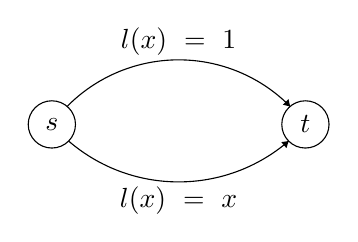
\begin{tikzpicture}[scale=0.1]
\tikzstyle{every node}+=[inner sep=0pt]
\draw [black] (18,-17.9) circle (3);
\draw (18,-17.9) node {$s$};
\draw [black] (50.2,-17.9) circle (3);
\draw (50.2,-17.9) node {$t$};
\draw [black] (19.94,-15.615) arc (135.3471:44.6529:19.905);
\fill [black] (48.26,-15.62) -- (48.05,-14.69) -- (47.34,-15.4);
\draw (34.1,-9.2) node [above] {$l(x)\mbox{ }=\mbox{ }1$};
\draw [black] (48.072,-20.011) arc (-49.23907:-130.76093:21.4);
\fill [black] (48.07,-20.01) -- (47.14,-20.15) -- (47.79,-20.91);
\draw (34.1,-25.7) node [below] {$l(x)\mbox{ }=\mbox{ }x$};
\end{tikzpicture}
\end{center}
    \caption{Pigou's example traffic routing problem, with a demand of $r_{(s,t)} = 1$}
\label{fig:Pigou}
\end{figure}

\medskip\noindent
\textbf{The input} to a traffic routing problem consists of:
\begin{itemize}
    \item A network $G = (V, E)$ of $|V|$ destinations (e.g., locations or servers) and $|E|$ links 
     \item A set of $k$ source-destination pairs $S=\{(s_1,t_1), \cdots (s_k,t_k)\}$ representing traffic demands
    \item A {rate} $r_i$ of traffic for each $(s_i,t_i)\in S$ representing the demanded amount of traffic from $s_i$ to $t_i$
    \item A {latency} function $l$ that assigns a per-edge function $l_e$ to each edge $e$ describing how adding traffic (i.e., congestion) to $e$ affects the time taken to travel across $e$. We can also think of $l$ as assigning per-path costs: for any path $p$ in the graph
        $$l_p(f) = \sum_{e\in P}l_e(f_e)$$ 
        We assume that $l$ is continuous, nonnegative, and nondecreasing.
\end{itemize}
In Figure~\ref{fig:Pigou}, we see a single source-destination input network with an example (linear) cost function with $r_{(s,t)} = 1$.

\medskip\noindent
\textbf{Solutions} correspond to flow assignments to the set of simple paths $P_i$ between $s_i$ and $t_i$ for all $i$. Note that our solutions assume \emph{nonatomic} entities: the flows we find may not be integral.
Intuitively, this means that the demand from one $s_i$ to $t_i$ is generated by an infinite number
of entities in the network, which allows us to reason about continuous, rather than discrete, functions.
%
To describe a flow assignment $f$, we can consider $f_p$, the flow on a single path $p \in P_i$ (this adds an equal amount of flow $f_p$ to all edges in $p$), as well as $f_e = \sum_p \sum_{e\in p} f_p$, the flow on edge $e$ (the sum of flow on all paths that use $e$).

A \emph{feasible} solution given such an input is an assignment of path flows such that the demand from $s_i$ to $t_i$ is met:
$$\forall 1 \le i \le k,~\sum_{p\in P_i} f_p = r_i$$
%
An \emph{optimal} (feasible) solution given such an input is the feasible flow assignment $f$ that minimizes the \textbf{total weighted latency cost}, or \textbf{social welfare latency cost} $C(f)$, where
$$C(f) = \sum_i\sum_{p\in P_i}l_p(f)f_p = \sum_{e\in E} f_el_e(f_e)$$

Intuitively, we are calculating the latency of each path of a given flow assignment, weighing 
each path's latency proportional to the amount of flow through the path. More concretely,
if we were to let flow represent the routes chosen by (infinitely many) users, $C(f)$ calculates the average latency over all users. Thus, when minimizing $C(f)$, some users may incur 
more latency so that other users can go faster: the optimal flow is the \emph{socially optimal} solution.
Note that there exists an optimal flow $f^*$ minimizing $C(f)$ because we assume $l$ is continuous and the set of feasible flows is compact.

In our running example (Figure~\ref{fig:Pigou}), a feasible flow is any flow that sends one unit from $s$ to $t$ (divided in any fashion between the top and bottom edges).
The optimal flow is the flow that sends half the traffic through the lower edge and half through the upper edge: the users on the lower edge only experience a latency of $1/2$, while the users on the upper edge experience a latency of $1$, making the total weighted latency cost $3/4$.

\subsection{Coordination Models and the Price of Anarchy}
Before we can create algorithms to solve the traffic routing problem, we must first assume a \emph{coordination model} for our traffic network.
There are two clear extremes: (1) centralized control, in which some entity (e.g., an air traffic controller) knows all traffic demands and routes accordingly, and
(2) decentralization, i.e., a complete \emph{lack} of coordination between
entities in the network.
In a centralized setting, there is a clear optimal solution, as shown in the previous section.
However, in a decentralized and uncoordinated model, the lack of coordination and the exercise of free will can result in
inefficiencies. 

\medskip
\textbf{The Price of Anarchy} (PoA) allows us to measure the inefficiencies of a decentralized model, and was first introduced by Koutsoupias and Papadimitriou in 1999~\cite{poa}. 
We treat the decentralized model as a game in which each individual optimizes for her own individual cost function $c$, allowing us to compute the achieved flow at the resulting Nash equilibrium (proven to exist if the cost functions are continuous)~\cite{wardrop,haurie,winsten}.
The PoA is defined as the ratio between the social welfare latency cost at the optimal flow, and the social welfare latency coast at the flow achieved at equilibrium.
(This is similar to how we measured the distance from optimal of an approximation algorithm in a limited computational power model, and of online algorithms in an incomplete information model.)

The set of flows at Nash equilibrium are defined such that for all $i$ source-destination pairs, all the paths from $s_i \to t_i$ have the minimum-possible cost with respect to $c$. In other words, in the selfish routing model, the (nonzero) flow paths at Nash equilibrium have equal path costs, and no user decreases her cost by choosing a different path:
$$\forall 0\le i \le k,~\forall p_1, p_2\in P_i~s.t.~f_{p_1} > 0~\text{and} f_{p_2} > 0,~ c_{p_1}(f) = c_{p_2}(f)$$
Note that this corresponds exactly to the solutions to the following (convex) program solvable in polynomial time:
$$NE = \min_f\Big(\sum_e \int_0^{f_e} c_e(t)dt\Big) \text{ subject to feasibility constraints}$$
whereas the flow optimizing the social welfare latency cost corresponds exactly to the (polynomial-time) solutions to the following (convex) program: 
$$SW = \min_f\Big(\sum_e f_el_e(f_e)\Big) \text{ subject to feasibility constraints}$$

\subsection{The Selfish Routing Model}
One example of an uncoordinated model is the \emph{selfish routing} model, in which all entities in the network are selfish and choose a route minimizing their individual latency without caring (or knowing) about the effects on other users~\cite{tardos}.
The selfish routing model corresponds to flows at a Nash equilibrium where each user optimizes her individual cost function
$c^s(f) = l(f)$.
Thus, the program optimized at Nash Equilibruim is
$$NE_{s} = \min_f\Big(\sum_e \int_0^{f_e} l_e(t)dt\Big) \text{ subject to feasibility constraints}$$

If we revisit our running example in Figure~\ref{fig:Pigou}, we note that the flow at Nash equilibrium corresponds to a flow that sends the entire unit of traffic through the bottom edge (the 0 flow through the top path has latency 1, and the unit flow through the bottom path will have latency 1).
Intuitively, each user routing from $s$ to $t$ will selfishly choose to take the bottom route because she will reason that the bottom route can have latency no worse than the top route. However, by doing so, the bottom route becomes more congested and leads to a total average latency $C(f) = 1$.
Thus, in Figure~\ref{fig:Pigou}, the price of anarchy $\rho$ is $\frac{1}{3/4} = \frac{4}{3}$.

We next describe and present the main results regarding the PoA in this (decentralized) selfish routing model, which will act as a basis to which we will compare traffic routing results in more recently formulated models.

\subsection{Main Results}
\begin{theorem}
    If $f$ is a flow at Nash Equlibrium for a given input set $(G, r, l)$ and $f^*$ is a feasible flow for $(G, 2r, l)$, then $C(f) \leq C(f^*)$
\end{theorem}

\begin{proof-sketch}
    In other words, this result suggests that the latency when all users of a network route with only their own interests in mind is utmost the optimal (minimum) latency for the same graph and latency functions
    with twice as much demand per path. 
    
    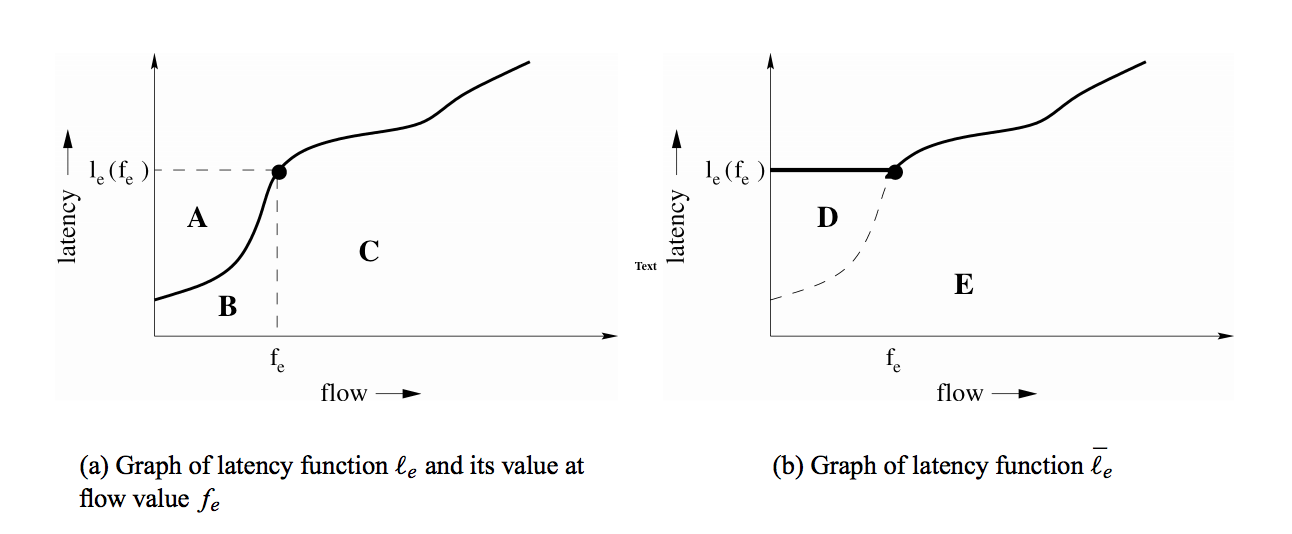
\includegraphics[width=1\textwidth]{graph}

    For any Nash Equilibrium solution $f$ for $(G, r, \ell)$ and any feasible solution $f^*$, we can draw the figures so that for each edge $e$ in $G$:
    
    The area $A+B$ represents the latency cost $C(f)$ of the Nash Equilibrium solution $f$ for $(G, r, \ell)$. The area $B+C$ represents the cost $C(f^*)$ of the feasible solution $f^*$ for $(G, 2r, \ell)$. Since the area $D+E$ is at most area $D$ more than area $B+C$, and area $D$ is less than area $A+B$, we know that $D+E-(B+C)\le D \le A+B $. This means that $B+C\ge D+E -(A+B)$. On the other hand $D+E\ge 2(A+B)$. Therefore, we have that $C(f^*)=(B+C)\ge 2(A+B)-(A+B)= A+B= C(f)$. Therefore we
    have the result that the latency of any Nash equilibrium flow for $(G, r, \ell)$ is no bigger than represents the latency of any feasible solution for $(G, 2r, \ell)$.
    The main idea of the proof for this theorem lies in that the subset if the area $C$ is at least as big as the area $A+B$. This is always true because the latency $\bar{\ell}_e$ is a nondecreasing function and thus the graph of latency function gives a shape that looks like a generalized trapezoid (in particular, a right generalized trapezoid lying on the horizontal axis). 
    %Then we can obtain the result based on the property of a trapezoid shape. Therefore, the cost of any feasible solution for $(G, 2r, \ell)$ is at least twice the cost $C(f)$ of any Nash equilibrium solution for $(G, r, \ell)$. Then the area under the black line from $0$ to $2f_e$ in subgraph (a) is at least $2C(f)-C(f)$ and thus larger than $C(f)$. 
   %The cost of any feasible solution for $(G, 2r, \ell)$, and the area under the black line from $0$ to $2f_e$ in subgraph (b) is at most $C(f)$ more than the cost of any feasible solution for $(G, 2r, \ell)$, and the area under the black line from $0$ to $2f_e$ in subgraph (a). So the area of the generalized trapezoid under the black line from $0$ to $2f_e$ is more than two times the area under the black line on the left side of $f_e$ in subgraph (b). 
    %$+E$ under the black line from $0$ to $2f_e$ in subgraph (b) represents the cost of any feasible solution for $(G, 2r, \ell)$. The area under the black line on the left side of $f_e$ in subgraph (a) represents the cost $C(f)$ of any Nash equilibrium solution for $(G, r, \ell)$. Note that since the area of t he area under the black line on the left side of $f_e$ in subgraph (a) is at least half of the dashed line, we know that the cost of any feasible solution for $(G, 2r, \ell)$, and the area under the black line from $0$ to $2f_e$ in subgraph (b) is at most $C(f)$ more than the cost of any feasible solution for $(G, 2r, \ell)$, and the area under the black line from $0$ to $2f_e$ in subgraph (a). So the area of the generalized trapezoid under the black line from $0$ to $2f_e$ is more than two times the area under the black line on the left side of $f_e$ in subgraph (b).
    % Vibhaa: might be helpful to add line segments/naming to the figure - also not sure if the black line on left side needs to be half of dashed line. Check 
    %also check notation
\end{proof-sketch}

\begin{theorem}
    If the edge latency functions are linear in that $l_e = a_ef_e + b_e$ for every edge $e \in E$, then the price of anarchy or $\rho(G, R,l) \leq 4/3$.
\end{theorem}

\begin{proof-sketch}
    The latency of any flow $f$ under these edge latency functions is $C(f) = \displaystyle \sum_e a_ef^2_e + b_ef_e$.

    Let's consider two flows $f$ and $f^*$ such that $f$ is at Nash Equlibrium in $(G, r, \ell)$ and $f^*$ is globally optimal for the same. We first consider optimally routing the first $r/2$ demand 
    across all source-destination pairs. It turns out that $f/2$ is optimal for $(G, r/2,\ell)$ when the edge latency functions are linear. This can be derived from the fact that paths with
    non-zero flow at a Nash Equlibrium have the same path latency while paths with non-zero flows at the global optimum have the same marginal cost of increasing the flow. Now, if we look at the cost
    $C(f/2)$ of routing this in terms of the latency of routing the flow $f$ at Nash Equlibrium, we notice that $C(f/2) = \displaystyle \sum_e \frac{1}{4}a_ef^2_e + \frac{1}{2}b_ef_e \geq \frac{1}{4}C(f)$
    from the above cost expression. Thus, in other words, routing the first $r/2$ optimally has a latency that is at least one-fourth of the latency of the Nash Equlibrium flow.
    %% Do we need the actual proof of the fact that $f/2$ is optimal for the half rate case - we could also just reference Lemmas 4.1 and 4.3?

    This leaves the remaining $r/2$ that needs to be routed optimally to route $f^*$ fully. To reason about this, let's look at a small $\delta r_i$ increase in flow from $s_i$ to $t_i$ that already carries $x$ units 
    of flow. For a convex latency function, we expect the increase in latency to be at least $\delta r_il'(x)$ where $l'$ if the minimum marginal increase in $C$. If we consider starting at the 
    optimal flow $f/2$ for the $r/2$ demand and increasing the flow on each path by a small $\delta r_i$, the subsequent increase in 
    latency across be all paths can be summed as  $\displaystyle \sum_{i = 1}^kl'(f/2)\delta r_i$. But, for linear edge latency functions, the marginal increase in latency on every edge at $f/2$ is exactly
    the latency of that edge at $f$. Thus, $l_e'(f/2) = l_e(f)$. Thus, setting $\delta = 1$ and increasing the rate by $r_i/2$ on every $s_i$, the overall increase in latency is  at least $\displaystyle \frac{1}{2}\sum_{i= 1}^kl(f)r_i
    = \frac{1}{2}C(f)$. The last part is by definition of $C(f)$. 
    
    In essence, routing the first $r/2$ demand optimally costs at least $C(f)/4$ and the next $r/2$ when augmented, costs at least another $C(f)/2$. In total, the optimal costs at least $\frac{3}{4}C(f)$. In other words,
    the flow at Nash Equilibrium has cost utmost $\frac{4}{3}C(f^*)$ where $f^*$ is the flow achieving optimal latency.
\end{proof-sketch}


\section{Alternative Models}
In this section, we present the models and results of a subset of recent coordination models for the traffic routing problem in the framework described in Section~\ref{sec:background}. These models propose a more nuanced (and perhaps more accurate) description of human behavior than the selfish model.
\subsection{Altruism and Spite}
We first consider an alternative model proposed by Chen and Kempe in 2008~\cite{chen}, which assumes that users are ``not entirely selfish.''
Chen and Kempe note that social experiments from both economic and psychology have shown humans do not behave rationally in a selfish manner; instead, our behavior is better modeled as either altruistic or malicious (spiteful).
Their model proposes a simple way to capture how people make decisions based upon how much latency a particular decision will cost other users: if someone is spiteful, she will want to increase others' latencies, and if she is altruistic, she will want to decrease their latencies.

\subsubsection{Formalization}
The formal Chen and Kempe model introduces a per-user \emph{altruism} coefficient $\beta$ and an individual user cost function
of $c^\beta_P$ for all paths $P$:
$$c^\beta_P(f) = \sum_{e \in P} \ell_e(f_e) + \beta\sum_{e\in P} f_e\ell'_e(f_e)$$
where $\ell_e(\cdot)$ is the latency function from the selfish routing setting, and $\ell'_e(\cdot)$ is the derivative with respect to $f_e$.

Note that the first term is exactly the individual user's objective to minimize from the selfish routing model (and thus the two models are equivalent when $\beta = 0$). The second term corresponds to the derivative of the social welfare latency cost on $p$ and is weighed by $\beta$; we use the derivative, rather than the value, of the social welfare cost on $p$ because each user only controls an infinitesimally small amount of the flow: if we were to use the value, a single user's choice would have no effect on the social welfare cost! 
Instead, a user can account for how she will affect the social welfare cost via the rate at which her choice of path affects other users.

If $\beta$ is negative, a user is spiteful: we know that adding a little more flow to $P$ will increase the social welfare cost of taking $p$ (the derivative $\ell'_e$ is positive), and since we negate this value, this lowers the user's perceived cost of taking $p$.
Conversely, if $\beta$ is positive, a user is altruistic: increasing flow increases the social welfare cost on $p$ and also the user's perceived cost of taking $p$.
We assume that $\beta$ ranges from -1 (extremely spiteful) to 1 (extremely altruistic), where $\beta=0$ corresponds to selfishness.
All analysis of the model assumes a particular distribution $\psi$ of $\beta$ for all users. 

Note that we can compare this model to the selfish model using the price of anarchy as a measure of inefficiency
because the altruistic model still achieves Nash equilibrium for any $\psi$ and cost function $c^\beta_P$. (Given any $\psi$, $c^\beta_P$ are continuous in the choice of path $P$ and in the distribution of other users' strategies $f$: Mas-Colell~\cite{mascolell} showed that any game of infinitely many players with cost functions continuous in the actions of the players and distribution of actions by other players has a Nash equilibrium.)
%Nash equilibrium is achieved at the flow solutions to the program
%$$NE^\beta = \min_f\sum_e\int_0^{f_e}c_e^\beta(t)dt \text{ subject to feasibility constraints}$$
We next present Chen and Kempe's core results about the price of anarchy of arbitrary networks when $\psi$ is uniform (all users have the same $\beta$ value), and briefly mention their results of non-uniform $\psi$ in parallel-link networks.

\subsubsection{Uniformly Distributed Altruism}
We first consider the case where $\psi$ is uniformly distributed, such that $\beta$ and therefore $c^\beta_P$ is the same for each user. We additionally assume that users tend to be altruistic, i.e., $\beta > 0$.
With these assumptions, we get a nice bound on the price of anarchy:
\begin{theorem}
For any $G$, demand rates $r$, and 
a uniform distribution $\psi$ with $\beta \in (0, 1]$,
if $\ell_e$ is nondecreasing and convex for all $e$, then the price of anarchy is bounded by 
    $$\rho(G,r,\ell,\psi) \le \frac{1}{\beta}$$
\end{theorem}

\begin{proof-sketch}
    Consider the two (convex) functions that we minimize for each of the user objectives
    for the altruistic model and the social welfare model (a cooperative model optimizing for the total overall latency).
    For simplicity, let $B(f)$ be the function minimized in the altruistic model; the second function is simply our social welfare cost $C(f)$.
    We can write these and manipulate them into comparable forms as follows:
    $$B(f) = \sum_e\int_0^{{f}_e}\Big(c_e^\beta(t)\Big)dt = 
        \sum_e\int_0^{{f}_e} \Big(\ell_e(t) + \beta t\ell'e(t)\Big)dt\text{ (by definition of $c^\beta_e$)}$$
    $$C(f) = \sum_ef_e\ell_e(f_e) = \sum_e\int_0^{f_e} \Big((t\ell_e(t))' \Big)dt 
        = \sum_e\int_0^{f_e} \Big(\ell_e(t) + tl'e(t)\Big)dt$$ 
    It is clear that for any feasible flow $f$, 
    $B(f) \le C(f) \le \frac{B(f)}{\beta} \text{ because $\beta\in(0,1]$}$.
    We now let $\hat{f}$ be the flow at Nash equilibrium and $f^*$ be the flow at optimum social welfare. Because these are the optimal flows for their respective objectives, we know that 
    $C(\hat{f}) \le \frac{B(\hat{f})}{\beta} \le \frac{B(f^*)}{\beta} \le \frac{C(f^*)}{\beta}$,
    proving that 
    $\rho(G,r,\ell,\psi) \le \frac{1}{\beta}$
\end{proof-sketch}

\subsubsection{Uniformly Distributed Spite}
Chen and Kempe then address the problem of spite: how (uniformly) spiteful can users be before $\rho$ becomes infinite?
It turns out that this depends on the type of latency function! Our analysis begins by reasoning about the price of anarchy of a given class ${L}$ of latency functions, 
$\rho(G,r,{L},\psi)$.

We find that the price of anarchy of a class of functions $L$ is lower-bounded by the worst possible price of anarchy (over all $\ell \in L$ ) achieved in a two-link, two-node network (such as in Figure~\ref{fig:Pigou}) routing $r$ demand with the following latency functions on its two edges:
$\ell_1(x) = \ell(x)$ and $\ell_2(x) = c^\beta{r} = \ell(r) +\beta r\ell'(r)$.

We refer to this specific two-link problem for a given input $(G,r,L,\psi)$ as $T_\beta$, and the maximum price of anarchy of this problem over all $\ell \in L$ as $\rho(T_\beta)$.
\begin{theorem}
For any $G$, demand rates $r$ and uniform distribution $\psi$ of $\beta \in (-1, 1]$,
    $$\rho(G,r,{L},\psi) \le \rho(T_\beta)$$
   i.e., the price of anarchy of a class of functions $L$ routing $r$ flow in $G$ is 
    bounded by the price of anarchy routing $r$ flow through the network $T_\beta$.
    \end{theorem}
\begin{proof-sketch}
    We give a brief overview of the proof technique here.
    Note that by definition, 
    the flow in $T_\beta$ at Nash equilibrium will route all demand $r$ on the edge with latency function $\ell_1(x) = c(x)$, whereas the socially optimal flow will route some flow $x$ on the edge with latency function $\ell_2 = c^\beta(r)$. This gives us the worst case for $\rho(T_\beta)$ given any $\ell \in L$ as
    $$\rho(T_\beta) = \max_{l\in{L}} \max_{x,r\ge 0} \frac{r\ell(r)}{x\ell(x) + (r-x)(c^\beta(r))}$$
    The proof proceeds by considering social welfare cost of the flow $f^*$ optimizing $C$. By unfolding the definition of $\rho(T_\beta$) to get a bound for $x\ell_e(x)$ for arbitrary $x$ and $r$, we can then apply this bound to each edge with $x = f^*_e$ and $r = \hat{f}_e$, where $\hat{f}$ is the optimizing flow at Nash equilibrium. 
    $$\forall x,r\ge 0,~ x\ell_e(x) \ge \frac{r\ell_e(r)}{\rho(T_\beta)}  + (x-r)c^\beta_e(r)
    \implies  f^*_e\ell_e(f^*_e) \ge \frac{\hat{f}_e\ell_e(\hat{f}_e)}{\rho(T_\beta)}  + (f^*_e-\hat{f}_e)c^\beta_e(\hat{f}_e)$$
    With some mathematical manipulation, we can derive a comparison of $C(f^*)$ to $B(\hat{f})$ satisfying the above bound:
    \begin{align*}
        C(f^*) = \sum_e f^*_e\ell_e(f^*_e) &\ge \sum_e \frac{\hat{f}_e\ell_e(\hat{f}_e)}{\rho(T_\beta)} + (f^*_e-\hat{f}_e)c^\beta_e(\hat{f}_e)\\
        &\ge \frac{C(\hat{f})}{\rho(T_\beta)} + \sum_e (f^*_e-\hat{f}_e)c^\beta_e(\hat{f}_e)
    \end{align*}
    Note that $\sum_e (f^*_e) c^\beta_e(\hat{f}_e) \ge \sum_e \hat{f}_ec^\beta_e(\hat{f}_e)$ by definition of $\hat{f}$ being a flow at Nash equilibrium (see Theorem~\ref{variational}).
    Thus, we get that 
        $$C(f^*) \ge \frac{C(\hat{f})}{\rho(T_\beta)}\implies \rho(T_\beta) \ge \frac{C(\hat{f})}{C(f^*)}$$
\end{proof-sketch}

Since we know how to bound $\rho(G,r,{L},\psi)$ by the (uniform) value of $\beta$, we can now determine at which values of $\beta$ this lower bound is infinite: how spiteful do users have to be to cause each other infinitely more suffering? The following result shows that if the latency functions are in the class $L_d =$ polynomials of degree $\le d$, the price of anarchy is bounded when $\beta$ is at least $\frac{-1}{d}$ (and is infinite when $\beta < \frac{-1}d$).
\begin{theorem}
    Let $L_d$ be the class of latency functions that are polynomials of degree $\le d$.
    For any $G$, demand rates $r$, $\ell \in L_d$, and uniform distribution $\psi$ with $\beta \in (\frac{-1}{d}, 1]$,
    $$\rho(G,r,\ell,\psi) \le \Big(\Big(\frac{1+\beta d}{1+d}\Big)^{1/d}\Big(\frac{1+\beta d}{1+d} + 1 + \beta d\Big)+ 1 + \beta d\Big)^{-1}$$
\end{theorem}
\begin{proof-sketch}
From Theorem 4, we know that 
$\rho(G,r,{L},\psi)$% \le \max_{l\in{L_d}} \max_{x,r\ge 0} \frac{r\ell(r)}{x\ell(x) + (r-x)(c^\beta(r))}$, where the RHS corresponds to 
    is bounded above by $\rho(T_\beta)$. Thus, we only need to consider how bad $\rho(T_\beta)$ can get given any $l\in L_d$.

    The key observation is that $\exists\lambda \in [0,1]$ s.t. $c^1(r\lambda) = c^\beta(r)$, where $c^1$ is the cost function with uniform altruism value $\beta=1$. This will allow us to reason about the amount of flow $r\lambda$ that the optimum solution will place on the link with latency function $l_1(x) = \ell(x)$, and precisely compute the price of anarchy in terms of $\beta$.

    Observe that a Nash equilibrium flow in a two-node two-link network $T_\beta$ routing $r$ units from the source to the destination will put all flow on the link with cost function $l_1(x) = \ell(x)$. By definition of $\lambda$, the solution optimizing social welfare will put $r\lambda$ flow on the first link with latency function $\ell_1(x) = \ell(x)$, and $r(1-\lambda)$ on the second link with latency function $\ell_2(x) = c^\beta(r)$. This gives us a bound on the price of anarchy:
    $$\rho(G,r\lambda,\ell,\psi) \le \rho(T_\beta) \le \Big(\frac{\lambda \ell(r\lambda)}{\ell(r)} + \Big(1-\lambda\Big)\Big(1+\frac{\beta r\ell'(r)}{\ell(r)}\Big)\Big)^{-1}$$

    To satisfy our observation, we need to make an appropriate choice of $\lambda$. To simplify our calculation of $\lambda$, we can, without loss of generality, consider latency functions $\ell(x) = ax^i$ for some $i \le d$ to represent all functions $\ell \in L_d$. We can then solve $c^1(r\lambda) = c^\beta(r)$ for $\lambda$ to get $\lambda = \Big(\frac{1+\beta i}{1+i}\Big)^{\frac{1}{i}}$.
    With this $\lambda$, we get that $\frac{\ell(r\lambda)}{\ell(r)} = \frac{1+\beta i}{1+i}$ and $\frac{\ell'(r)}{\ell(r)} = \frac{i}{r}$. We can plug these values into the bound to get:
    $$\rho(G,r,\ell,\psi) = \rho(G,\lambda r, \ell,\beta=1) \le \Big(\Big(\frac{1+\beta i}{1+i}\Big)^{1/i}\Big(\frac{1+\beta i}{1+i} + 1 + \beta i\Big)+ 1 + \beta i\Big)^{-1}$$
    This is increasing in $i$, giving us the worst-case bound when $i=d$:
$$\Big(\Big(\frac{1+\beta d}{1+d}\Big)^{1/d}\Big(\frac{1+\beta d}{1+d} + 1 + \beta d\Big)+ 1 + \beta d\Big)^{-1}$$
\end{proof-sketch}

\subsubsection{Arbitrarily Distributed Altruism}
Chen and Kempe go on to extend their analysis to when users have an arbitrary distribution $\psi$ of altruism (with no spiteful users) in \emph{parallel link networks}, networks with only two nodes (a source and destination) and parallel edges running between the nodes. 
We briefly mention their results here, but direct the reader to the paper for a more detailed proof.
%, which have only one demand source-sink pair $(s,t)$ and (parallel) edges only between $s$ and $t$.
%Stackleberg routing shown to have unlimited PoA in single-commodity networks
Their main result mirrors that of uniform altruism:
\begin{theorem}
    Given any parallel link network $G$, demand rates $r$, altruism density function $\psi$ with average altruism $\bar{\beta}$ and non-negative support (no spiteful users), and convex and non-decreasing cost functions $\ell_e$,
   $\rho(G,r,\ell,\psi) \le \frac{1}{\bar{\beta}}$
\end{theorem}
Finally, Chen and Kempe comment on the restriction to $\beta \ge 0$: if even a small fraction of users are spiteful, these users can, in some networks instances, lead to an price of anarchy much greater than 1 regardless of the value of $\bar{\beta}$.

\subsection{Risk Aversion}
The second model we consider accounts for the
tendency of users to pick routes with less variation in latency even if it comes at the cost of some added
latency on the paths chosen. This increase in latency can be quantified as the {\em{price of risk-aversion}}
which is the worst-case ratio of the latency or cost at a risk-averse Nash Equilibrium to that at a risk-neutral
Nash equilibrium or one where users are indifferent to variations in the latency itself.

%% The key result that we will be focussing on here is one where we show that the latency bounds in this context
%% is effectively the price of anarchy times the price of risk-aversion which intuitiveluy makes sense.

\subsubsection{Formalization} The {\textbf{formal model}} introduced in Lianeas et.al \cite{risk-averse} defines 
a risk aversion coefficient $\gamma$ that quantifies the users' tendency to prefer paths with less variability. 
A higher $\gamma$ means that one is more risk averse. The edge costs $c_e(x_e)$ now have a deterministic part 
or $l_e(x_e)$ and a noise modelled by a random variable $\xi_e(x_e)$. The latter is assumed to be independent across edges 
and has expectation $0$ and variance $\upsilon_e(x_e)$ for $x_e$ flow allowing us to sum them up over a path. To simplify 
the analysis, the model also defines $\upkappa$ to bound the variance-to-mean latency ratio. In other words, 
$\upsilon_e(x_e) \leq \upkappa l_e(x_e)$.
%Now,
%the expected latency and variance ($\upsilon_p$) on a path can be summed across all the edges. Consequently, our problem
%instance is $(G,r,l,\upsilon,\gamma)$ and we focus on $r = 1$ to simplify our analysis.

The cost function or the {\textbf{objective}} that every user is now optimizing for is of the form
$$c_p(f) = \sum_{e \in p}l_e(f_e) + \gamma \sum_{e \in p}\upsilon_e(f_e)$$
This function is assumed to be non-decreasing. Intuitively, the mean is identical to the original price of anarchy formulation
while the second term accounts for variance. Minimizing this implies that we want to minimize the variance depending on the
value of the risk coefficient itself.

If the maximum cost $C(x)$  across some set of nash equlibria flows $x$ for the given problem instance 
that is restricted to some family of inputs and a fixed $\upkappa$, the {\textbf{price of risk-aversion}} is now defined as the
ratio $C(x)/C(z)$. Here $C(z)$ is the cost associated with some risk-neutral nash equilibrium $z$. 
In the following section, we look at bounding this price of risk-aversion. Note that this can be viewed as contributing a 
multiplicative factor to the price of anarchy in the overall change to the latency or cost of the system. We first prove a 
more basic result from an older paper on this topic \cite{risk-averse-background} and then proceed to the main result on the price
of risk-aversion for 
a special family of latency functions that are $(\lambda, \mu)$ smooth. Note that additional results can be proved for special classes
of graph topologies which can be found in the original paper \cite{risk-averse}.


%%\begin{itemize}
%%
%%\item Mean-variance objective 
%%\begin{itemize}
%%    \item additive factor allowing you to reason about optimal
%%    \item assumed to be non-decreasing for the same reasons as the original model
%%    \item the mean is similar to the old function we were minimizing or the latency alone 
%%    \item but now we have an additional term that we are trying to minimize the variance depending on our risk-aversion coefficient
%%    \item Players try to optimize for this mean-variance objective which takes both the above aspects into account which is collectively called path-cost
%%\end{itemize}
%%
%%\item Social Cost of a flow - sum of the expected latencies of all players $C(f) = \displaystyle \sum_{p \in P} f_pl_p(f) = 
%%\sum_{e \in E}f_el_e(f_e)$. This reoves the dependency on per user risk aversion coefficients and rather takes a look at the system as a whole.
%%
%%\item Define PRA 
%%\begin{itemize} 
%%    \item $\upkappa$ definition -  variance to mean ratio and maximum bound on it
%%    \item Maximum cost across some set of nash equlibria flows $x$ for the given problem instance that belongs 
%%	to a certain class of instances and $\upsilon(x) \leq \upkappa l(x)$
%%    \item note about results depending on the graph topology
%%\end{itemize}
%%\end{itemize}
%%


\subsubsection{Main Results}
\begin{theorem}
    If a flow $f$ is at a risk averse nash equlibrium and $f^*$ is any other flow, then $fC(f)\leq f^*C(f)$. 
    \label{variational}
\end{theorem}

\begin{proof}
    By definition, any flow at Nash Equilibrium routes on paths with minimum cost or only sends flow on a given path if its cost is less than
    the cost of sending the same flow on some other path. Thus, for a fixed demand and fixed path costs determined by $C(f)$, $f^*$ differs from $f$ in 
    atleast moving some $\epsilon$ flow from one lower cost path to another higher cost one which increases the total overall cost. 
    Consequently, let's say we have a flow $x$ that is a risk averse Nash Equlibrium 
    for the cost function $c_e = l_e(x_e) +\gamma \upsilon_e(x_e)$. If $z$ is a risk neutral Nash Equilibirium, it is still feasible for the risk averse
    mean-variance cost function, but is not the equilibrium in that scenario. By the above description and costs written as the sum across edges, we have
    $$\sum_{e \in E}x_e(l_e(x_e) + \gamma \upsilon(x_e)) \leq \sum_{e \in E} z_e(l_e(x_e) + \gamma \upsilon_e(x_e))$$
\end{proof}

\begin{definition}
    A latency function $l(x)$ is $(\lambda, \mu)$-smooth if for all $x, y \geq 0$ $$ yl(x) \leq \lambda yl(y) + \mu x l(x)$$
    
    This is a particular instance of smoothness definitions for functions that allows us to show bounds on the price of risk-aversion for such restricted families of functions. 
\end{definition}

\begin{theorem}
    The set of instances with latency functions ${l_e}_{e \in E}$ that are $(1,\mu)$-smooth around any risk-averse nash equilibrium $x_e$ for all $e \in E$ have price of risk-aversion
    $\leq \displaystyle \frac{(1 + \gamma \upkappa)}{(1 - \mu)}$
\end{theorem}

\begin{proof}
    This proof involves separating the edges into two sets $A$ and $B$ where $A$ contains edges whose flow $x_e$ in the risk-averse nash equilibrium is utmost the flow on the same edge
    $z_e$ in the risk-neutral nash equilibrium and $B$ contains the rest of the edges. $x$ continues to be a risk-averse nash equilibrium while $z$ is a risk-neutral one. 
    
    Let's consider the edges in $A$. We know that by definition, $\sum_{e \in A}l_e(x_e) \leq \sum_{e \in A}l_e(z_e)$. In turn this means 
    $$\sum_{e \in A}(1 + \gamma\upkappa)z_el_e(x_e) \leq \sum_{e \in A}(1 + \gamma \upkappa)z_el_e(z_e)$$.

    Let's similarly consider the edges in $B$. By the definition of $(1, \mu)$-smoothness, we have $$\sum_{e \in B}z_el_e(x_e) \leq \sum_{e \in B}z_el_e(z_e) + \mu x_el_e(x_e)$$.
    
    Together, the last two statements mean that (adding some terms two both of them to encompass all the edges in each type of term), 
    $$\sum_{e \in A}(1 + \gamma\upkappa)z_el_e(x_e) +  \sum_{e \in B}z_el_e(x_e) \leq \sum_{e \in E}z_el_e(z_e) + 
    \sum_{e \in E} \mu x_el_e(x_e) + \sum_{e \in E}(1 + \gamma \upkappa)z_el_e(z_e) = (1 + \gamma \upkappa)C(z) + \mu C(x) $$

    Now, if we are able to show that the total social cost $C(x)$ of the risk averse nash equilibrium flow is somehow utmost the expression above, we have established our proof
    by rearranging the terms, because the price of risk-aversion in this case is given by $C(x)/C(z)$. 

    To establish this, let's take the expression from the Proof of Theorem \ref{variational} and use $C(x) = \sum_{e \in E} x_el_e(x_e)$ as well as separate edges by sets $A$ and $B$, we have 
    $$C(x) + \sum_{e \in A} x_e\gamma\upsilon_e(x_e) + \sum_{e \in B} x_e\gamma\upsilon_e(x_e) \leq \sum_{e \in A} z_e\gamma\upsilon_e(x_e) + \sum_{e \in B} z_e\gamma\upsilon_e(x_e) + \sum_{e \in E} z_el_e(x_e)$$
    By the definitions of $A$ and $B$, we can extract the sum of second and third terms from the left hand side and the second term on the right hand size, because the former is larger than the latter
    and can't contribute to this inequality. If we separate the last term on the right into sets $A$ and $B$ and apply $\upsilon_e(x_e) \leq \upkappa l_e(x_e)$, we effectively are left with
    $$C(x) \leq \sum_{e \in A}(1 + \gamma\upkappa)z_el_e(x_e) +  \sum_{e \in B}z_el_e(x_e) \leq (1 + \gamma \upkappa)C(z) + \mu C(x) $$
    which proves exactly what we need. 
\end{proof}

\XXX { single line about how special case of POA can be extracted and maybe brief mention of other result??}

\subsection{Diverse in Interests}\label{sec:diversity}

The third class of alternative models we consider is a generalization of the altruistic model and the risk-averse model that we have discussed in previous sections. This class is characterized by the diverse selfish behavior by its heterogeneous agents. Each agent pursues their own different selfish goal, resulting in a routing solution of the whole network. 

Diverse selfish routing models are useful because they help us understand how we can leverage policies and natural diversity of goals in a network to increase the social welfare and efficiency of the network as a whole. For example, tolls can help increase the social welfare. For example, Beckmann et. al. showed that tolls can help implement the social optimum as an equilibrium, when agents all have the same goal towards a linear combination of time and money \cite{beckmann1956studies}.

However, there is some ambiguity in measuring the optimality of any outcome of the whole network with diverse selfish behavior, because by definition, the objective function has changed from the objective of selfish routing with no agent heterogeneity and thus only one criterion. There are thus multiple reasonable ways to characterize the social welfare of a diverse routing network. We will discuss the model adopted by Cole, Lianeas and Nikolova and their newly published results in 2018 \cite{ijcai2018-24}.

\subsubsection{Model}

We have the same routing network with multiple source-destination pairs and continue with all our previous notations, except that we have included two criteria the players consider in the objective function.

Each agent wants to minimize their own cost $c$, which is a sum of two terms associated with two criteria. Let $\ell_P$ denote the cost of the first criterion (e.g., the latency) over some path $P=(s_i, t_i)$, and $\sigma_P$ be the cost of the second criterion, referred to as the {\it deviation function}. Then given a routing $f$ of the network, the cost of that path is given by $c_p = \ell_P+\omega\cdot \sigma_P=\sum_{e\in P} \ell_e(f_e)+ \sum_{e\in P}\sigma_e(f_e)$\XXX{LYT:
are you missing the diversity parameter here?}, where $\omega$ is the {\it diversity parameter}.

Note that the latency function has all the properties as we assumed in previous sections, while the deviation function $\sigma_e(x)$ is assumed to be continuous by not necessarily non-decreasing. However, the function $\ell_e+\omega\cdot \sigma_e$ must be non-decreasing. These assumptions are consistent with our previous risk-averse model in Section 3.2, because if $\sigma_e$ models the variance, then $\sigma_e$ could be decreasing in the flow.

Cole et. al. measures the effect of diversity against the resulting flow of a homogeneous agent population of the same size. The homogeneous agent population has the single diversity parameter $\bar{r}=\int rf(r)d r$. 

For a discrete distribution of $n$ discrete values $r_1^k, \dots, r_n^k$, the demand $d_k$ is a vector $d_k=(d_1^k, \dots, d_n^k)$ where each $d_i^k$ denotes the total demand of commodity $k$ with diversity parameter $r_i^k$ and $d^k$ denote commodity $k$'s total demand $d^k=\sum_{i=1}^n d_i^k$. For a heterogeneous equilibrium flow vector $g$, the {\it heterogeneous total cost} of commodity $k$ is denoted by $C^{k,ht}(g)=\sum_{j=1,\dots, n} d_j^k c^{k, r_j^k}(g)$, where $c^{k, r_j^k}(g)$ denotes the common cost at equilibrium $g$ for players of diversity parameter $r_j^k$ in commodity $k$. The heterogeneous total cost of $g$ is then $C^{ht}(g)=\sum_{k\in K} C^{k,ht}(g)$. 

For the corresponding homogeneous equilibrium flow $f$, i.e. the instance with diversity parameter $\bar{r}^k$, where $\bar{r}^k$ denotes the average diversity parameter for commodity $k$, players of commodity $k$ share the same cost $c^{\bar{r}^k}(f)$. Then, the homogeneous total cost of commodity $k$ under $f$ is $C^{k,hm}(f)=d_kc^{\bar{r}^k}(f)$, and the homogeneous total cost of $f$ is $C^{hm}(f)=\sum_{k\in K} C^{k,hm}(f)$. 


\subsubsection{Results}
Let $g$ denote an equilibrium flow for the heterogeneous agent population and $f$ an equilibrium flow for the corresponding homogeneous agent population. Let $C^{ht}(g)$ denote the cost of flow $g$ and $C^{hm}(f)$ the cost of flow $f$. 

A {\it multi-commodity network} is consistent with all our previous models. We also introduce the definition of a {\it single-commodity network} as a network whose edges all belong to some single source-destination path as only these edges are going to be used by the equilibria and thus all other edges can be discarded. We present the following main results.

\begin{definition}
A directed $s-t$ network $G$ is {\it series-parallel} if it consists of a single edge $(s, t)$, or it is formed by the series or parallel composition of two series-parallel networks with terminals $(s_1, t_1)$ and $(s_2, t_2)$, respectively.
\end{definition}

The theorem below essentially states that for single-commodity networks, diversity is always helpful in a single-commodity series parallel network.

\begin{theorem}
For any $s-t$ series-parallel network $G$ with a single commodity, we have $C^{ht}(g)\le C^{hm}(f)$.
\label{diverse1}
\end{theorem}

\begin{proof-sketch}

The key observation is that since $f$ and $g$ route the same amount of flow from the unique source to the unique sink, there must be a path $P$ where $f$ sends no less flow along than $g$ does. Since the network is series-parallel, for every edge $e$ in $P$, $f_e \ge g_e$. This is true because a path in a series-parallel network can be broken up into some series-parallel parts in series and some series-parallel parts in parallel, which recursively breaks down to a simple series of edge(s). Hence for any $r\in [0, r_{\max}]$, we have $c_P^r(f)\ge c_P^r(g)$. This simultaneously also means that $g$ could route more flow on $P$ but it doesn't, implying that there is no incentive for $g$ to switch the flow it sends on other paths to path $P$ under the same diversity parameter. Therefore $c^r(g)\le \sum_{e\in P} \ell_e(g_e)+r\sum_{e\in P}\sigma_e(g_e)$. Then $C^{ht}(g)\le \sum_{i=1}^k d_i(\sum_{e\in P} \ell_e(g_e)+r_i\sum_{e\in P}\sigma_e(g_e))=\ell_p(g)+\bar{r}\sigma_P(g)$ which is exactly the cost of the homogeneous equilibrium flow $f$.
\end{proof-sketch}


\begin{theorem}
For any $s-t$ non-series-parallel network $G$ with a single commodity, there exists cost functions $C$ for which $C^{ht}(g)> C^{hm}(f)$.
\label{diversethm2}
\end{theorem}

\begin{proof-sketch}
If $G$ is not series-parallel then the Braess graph can be embedded in it \cite{Valdes:1979:RSP:800135.804393}, and there are edge functions such that heterogeneous equilibrium flow has a larger cost than homogeneous equilibrium flow. Detailed example can be found in \cite{ijcai2018-24}.
%The key reason is that for a series-parallel network, if two flows $|f|\ge |g|$, then there must be a parallel part $P_1$ of the network where $f$ sends more flow than $g$ on. This must be true because we can trivially think of the whole network as $P_1$. Since in a series-parallel network, we can decompose $P_1$ into some
\end{proof-sketch}

This theorem essentially states that for single-commodity networks, diversity is always helpful only in a series-parallel network. Together with Theorem \ref{diverse1}, we know that the series-parallel structure is a sufficient and necessary condition for diversity to always be helpful.

Now we discuss our main results for multiple commodity network. We use {\it average-respecting demand} to refer to the property that for any commodity $i,j: \bar{r}^i=\bar{r}^j$. 

A multi-commodity network $G$ can be decomposed in subnetworks $G_i$'s that each contains all the vertices and edges of $G$ that belong to a simple $s_i-t_i$ path for commodity $i$. WLOG, we assume these $G_i$ are acyclic.

\begin{definition}
A multi-commodity network $G$ is {\it block-matching} if for every $i$, $G_i$ is series-parallel, and for every $i, j$, $G_i$ and $G_j$ are block-matching, respectively.
\end{definition}

The next theorem states that for multi-commodity networks, diversity is always helpful on any block-matching network with average-respecting demand. 

\begin{theorem}
For any $k$-commodity block-matching network with average-respecting demand, $C^{ht}(g)\le C^{hm}(f)$.
\label{diverse2}
\end{theorem}

\begin{proof-sketch}

The key idea is that for any block representation of a subnetwork $G_i=s_i B_1 v_1\dots v_{b_i-1} B _{b_i}t_i$ for some commodity $i$, because $G$ is block-matching, for any block $B_j$ connecting $v_{j-1}$ and $v_j$ , any other commodity $j$ either contains block $B_j$ as a block in its block representation or contains none of the edges of $B_j$. This implies that under any routing of the demand, either all of $j$'s demand goes through $B_j$ or none of it does. So the total traffic routed by $f$ and $g$ are the same from $v_{j-1}$ to $v_j$. So if restricted to the block, the cost of the heterogeneous equilibrium is less than or equal to that of the homogeneous equilibrium; then the theorem is a result of summing over every block of all commodities.
\end{proof-sketch}



\begin{theorem}
For any $k$-commodity network, if diversity helps for every instance on $G$ with average-respecting demand, we have $C^{ht}(g)\le C^{hm}(f)$, then $G$ is a block-matching network.
\end{theorem}

\begin{proof-sketch}
The proof is by contradiction. First, by our Theorem \ref{diversethm2} for single-commodity network, each subnetwork $G_i$ in our multi-commodity network must be a series-parallel network, otherwise we can use the same counterexample as for Theorem \ref{diversethm2}. Then since we can prove that any two commodities $i$ and $j$, any block of $G_i$ and any block of $G_j$ either have the same terminals and direction or their terminals has no intersection, we know that $G$ is block-matching. The detailed proof assumes the conditions does not hold and constructs demand and edge functions where diversity hurts to contradict the assumption. See \cite{ijcai2018-24}.
\end{proof-sketch}

This theorem essentially states that for multi-commodity networks, diversity is always helpful only on any block-matching network with average-respecting demand. Together with Theorem \ref{diverse2}, we know that the block-matching structure is a sufficient and necessary condition for diversity to always be helpful in a multi-commodity network.

\section{Discussion}\label{sec:discussion}

\begin{table}
\begin{center}
 \begin{tabular}{|c | c | c|} 
 \hline
 Name & Objective & Results \\
 \hline\hline
     Social Welfare & $SW = \min_f\Big(\sum_e f_el_e(f_e)\Big)$ & PoA = 1 (optimal by definition) \\
 \hline
     Selfish & $NE^s = \min_f\Big(\sum_e\int_0^{f_e} l_e(t)dt\Big)$ & TODO\\
 \hline
     Altruistic & $NE^\beta = \min_f\Big(\sum_e\int_0^{f_e} l_e(t) + \beta tl'e(t)dt\Big)$ & TODO\\
\hline
     Risk-averse & $NE^\gamma = \min_f\Big(\sum_e\int_0^{f_e} l_e(t) + \gamma\upsilon(t)dt\Big)$ & TODO\\
\hline
     Diverse Interests & $NE^\omega = \min_f\Big(\sum_e\int_0^{f_e} l_e(t) + \omega\cdot \sigma_e dt\Big)$ & TODO\\
     & where $l$ and $\sigma$ are the costs of two general criterion &\\
\hline
\end{tabular}
\end{center}
\end{table}

\subsection{Extensions}
Clearly the models we present are a miniscule subset of all potential models for human behavior; 
furthermore, they are coarse-grained and oversimplistic in comparison with the complexity of the human
brain. As understanding of the neurophysiological aspects of human behavior improves, we hope to see a matching evolution in the precision and accuracy of these models for traffic routing as well.




\bibliography{paper}
\bibliographystyle{acm}

\end{document}
